% ============================================================
%  Information Theory --- Module 2 --- ALL DIAGRAMS (merged)
%  Compile with pdfLaTeX.  Each diagram starts on its own page.
%  Auto-merged from Information_Theory_Module2_Solutions.md
% ============================================================
\documentclass[11pt]{article}
\usepackage[a4paper,margin=1.5cm]{geometry}
\usepackage{amsmath}
\usepackage{tikz}
\usetikzlibrary{automata,positioning,arrows.meta,trees,calc}
\usepackage{forest}
\usepackage{pgfplots}
\pgfplotsset{compat=1.18}
\setlength{\parindent}{0pt}
\title{\textbf{Information Theory --- Module 2}\\[2pt] All Diagrams (TikZ / forest / pgfplots)}
\author{}
\date{}
\begin{document}
\maketitle

% ---------- Q11 : diagram 1 ----------
\clearpage
\section*{Q11 --- diagram 1}
\begin{center}
\begin{forest}
for tree={grow'=east, parent anchor=east, child anchor=west, edge={-Stealth},
          l sep=14mm, s sep=4mm, font=\footnotesize}
[{root}
  [{$S_1=0$}, edge label={node[midway,above,font=\tiny]{0}}]
  [{$\bullet$}, edge label={node[midway,below,font=\tiny]{1}}
    [{$S_2=10$}, edge label={node[midway,above,font=\tiny]{0}}]
    [{$\bullet$}, edge label={node[midway,below,font=\tiny]{1}}
      [{$S_3=110$}, edge label={node[midway,above,font=\tiny]{0}}]
      [{$S_4=1110$}, edge label={node[midway,below,font=\tiny]{1}}]]]
]
\end{forest}
\end{center}

% ---------- Q13 : diagram 2 ----------
\clearpage
\section*{Q13 --- diagram 2}
\begin{center}
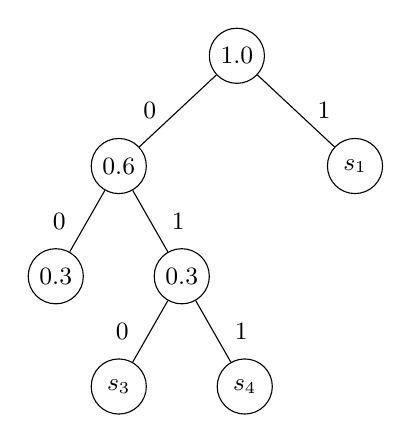
\begin{tikzpicture}[level distance=14mm,
  level 1/.style={sibling distance=30mm},
  level 2/.style={sibling distance=16mm},
  every node/.style={draw,circle,inner sep=1.5pt,minimum size=7mm,font=\small}]
\node {1.0}
  child {node {0.6}
    child {node {0.3} edge from parent node[left,draw=none]{0}}   % s2 = 00
    child {node {0.3}                                              % -> 010,011
      child {node {$s_3$} edge from parent node[left,draw=none]{0}}
      child {node {$s_4$} edge from parent node[right,draw=none]{1}}
      edge from parent node[right,draw=none]{1}}
    edge from parent node[left,draw=none]{0}}
  child {node {$s_1$} edge from parent node[right,draw=none]{1}};  % s1 = 1
\end{tikzpicture}
\end{center}

% ---------- Q14 : diagram 3 ----------
\clearpage
\section*{Q14 --- diagram 3}
\begin{center}
\begin{forest}
for tree={grow'=east, parent anchor=east, child anchor=west, edge={-Stealth},
          l sep=16mm, s sep=5mm, font=\small}
[{$1.0$}
  [{$s_1$ (0.7) $\to$ 0}, edge label={node[midway,above,font=\tiny]{0}}]
  [{$0.3$}, edge label={node[midway,below,font=\tiny]{1}}
    [{$s_2$ (0.15) $\to$ 10}, edge label={node[midway,above,font=\tiny]{0}}]
    [{$s_3$ (0.15) $\to$ 11}, edge label={node[midway,below,font=\tiny]{1}}]]
]
\end{forest}
\end{center}

% ---------- Q14 : diagram 4 ----------
\clearpage
\section*{Q14 --- diagram 4}
\begin{center}
\begin{forest}
for tree={grow'=east, parent anchor=east, child anchor=west, edge={-Stealth},
          l sep=14mm, s sep=2mm, font=\footnotesize}
[{$1.0$}
  [{AA (0.49)}, edge label={node[midway,above,font=\tiny]{0}}]
  [{$0.51$}, edge label={node[midway,below,font=\tiny]{1}}
    [{$0.21$}, edge label={node[midway,above,font=\tiny]{0}}
      [{AB (0.105)}, edge label={node[midway,above,font=\tiny]{0}}]
      [{AC (0.105)}, edge label={node[midway,below,font=\tiny]{1}}]]
    [{$0.30$}, edge label={node[midway,below,font=\tiny]{1}}
      [{BA (0.105)}, edge label={node[midway,above,font=\tiny]{0}}]
      [{$0.195$}, edge label={node[midway,below,font=\tiny]{1}}
        [{CA (0.105)}, edge label={node[midway,above,font=\tiny]{0}}]
        [{$0.09$}, edge label={node[midway,below,font=\tiny]{1}}
          [{$0.045$}, edge label={node[midway,above,font=\tiny]{0}}
            [{BB (0.0225)}, edge label={node[midway,above,font=\tiny]{0}}]
            [{BC (0.0225)}, edge label={node[midway,below,font=\tiny]{1}}]]
          [{$0.045$}, edge label={node[midway,below,font=\tiny]{1}}
            [{CB (0.0225)}, edge label={node[midway,above,font=\tiny]{0}}]
            [{CC (0.0225)}, edge label={node[midway,below,font=\tiny]{1}}]]]]]]
]
\end{forest}
\end{center}

% ---------- Q15 : diagram 5 ----------
\clearpage
\section*{Q15 --- diagram 5}
\begin{center}
\begin{forest}
for tree={grow'=east, parent anchor=east, child anchor=west, edge={-Stealth},
          l sep=14mm, s sep=2mm, font=\footnotesize}
[{$1.0$}
  [{$0.58$}, edge label={node[midway,above,font=\tiny]{0}}
    [{$0.33$}, edge label={node[midway,above,font=\tiny]{0}}
      [{C (0.18)}, edge label={node[midway,above,font=\tiny]{0}}]
      [{D (0.15)}, edge label={node[midway,below,font=\tiny]{1}}]]
    [{$0.25$}, edge label={node[midway,below,font=\tiny]{1}}
      [{$0.15$}, edge label={node[midway,above,font=\tiny]{0}}
        [{F (0.08)}, edge label={node[midway,above,font=\tiny]{0}}]
        [{$0.07$}, edge label={node[midway,below,font=\tiny]{1}}
          [{G (0.05)}, edge label={node[midway,above,font=\tiny]{0}}]
          [{H (0.02)}, edge label={node[midway,below,font=\tiny]{1}}]]]
      [{E (0.10)}, edge label={node[midway,below,font=\tiny]{1}}]]]
  [{$0.42$}, edge label={node[midway,below,font=\tiny]{1}}
    [{A (0.22)}, edge label={node[midway,above,font=\tiny]{0}}]
    [{B (0.20)}, edge label={node[midway,below,font=\tiny]{1}}]]
]
\end{forest}
\end{center}

% ---------- Q15 : diagram 6 ----------
\clearpage
\section*{Q15 --- diagram 6}
\begin{center}
\begin{forest}
for tree={grow'=east, parent anchor=east, child anchor=west, edge={-Stealth},
          l sep=14mm, s sep=2mm, font=\footnotesize}
[{$1.0$}
  [{A (0.22)}, edge label={node[midway,above,font=\tiny]{0}}]
  [{$0.53$}, edge label={node[midway,above,font=\tiny]{1}}
    [{B (0.20)}, edge label={node[midway,above,font=\tiny]{0}}]
    [{C (0.18)}, edge label={node[midway,above,font=\tiny]{1}}]
    [{D (0.15)}, edge label={node[midway,below,font=\tiny]{2}}]]
  [{$0.25$}, edge label={node[midway,below,font=\tiny]{2}}
    [{E (0.10)}, edge label={node[midway,above,font=\tiny]{0}}]
    [{F (0.08)}, edge label={node[midway,above,font=\tiny]{1}}]
    [{$0.07$}, edge label={node[midway,below,font=\tiny]{2}}
      [{G (0.05)}, edge label={node[midway,above,font=\tiny]{0}}]
      [{H (0.02)}, edge label={node[midway,above,font=\tiny]{1}}]
      [{dummy (0)}, edge label={node[midway,below,font=\tiny]{2}}]]]
]
\end{forest}
\end{center}

% ---------- Q16 : diagram 7 ----------
\clearpage
\section*{Q16 --- diagram 7}
\begin{center}
\begin{forest}
for tree={grow'=east, parent anchor=east, child anchor=west, edge={-Stealth},
          l sep=14mm, s sep=2mm, font=\footnotesize}
[{$1.0$}
  [{A (0.22)}, edge label={node[midway,above,font=\tiny]{0}}]
  [{B (0.20)}, edge label={node[midway,above,font=\tiny]{1}}]
  [{C (0.18)}, edge label={node[midway,above,font=\tiny]{2}}]
  [{$0.40$}, edge label={node[midway,below,font=\tiny]{3}}
    [{D (0.15)}, edge label={node[midway,above,font=\tiny]{0}}]
    [{E (0.10)}, edge label={node[midway,above,font=\tiny]{1}}]
    [{F (0.08)}, edge label={node[midway,above,font=\tiny]{2}}]
    [{$0.07$}, edge label={node[midway,below,font=\tiny]{3}}
      [{G (0.05)}, edge label={node[midway,above,font=\tiny]{0}}]
      [{H (0.02)}, edge label={node[midway,above,font=\tiny]{1}}]
      [{dummy (0)}, edge label={node[midway,above,font=\tiny]{2}}]
      [{dummy (0)}, edge label={node[midway,below,font=\tiny]{3}}]]]
]
\end{forest}
\end{center}

% ---------- Q17 : diagram 8 ----------
\clearpage
\section*{Q17 --- diagram 8}
\begin{center}
\begin{forest}
for tree={grow'=east, parent anchor=east, child anchor=west, edge={-Stealth},
          l sep=14mm, s sep=2mm, font=\footnotesize}
[{$1.0$}
  [{$0.50$}, edge label={node[midway,above,font=\tiny]{0}}
    [{S0 (0.25)}, edge label={node[midway,above,font=\tiny]{0}}]
    [{$0.25$}, edge label={node[midway,below,font=\tiny]{1}}
      [{S2 (0.125)}, edge label={node[midway,above,font=\tiny]{0}}]
      [{S3 (0.125)}, edge label={node[midway,below,font=\tiny]{1}}]]]
  [{$0.50$}, edge label={node[midway,below,font=\tiny]{1}}
    [{S1 (0.25)}, edge label={node[midway,above,font=\tiny]{0}}]
    [{$0.25$}, edge label={node[midway,below,font=\tiny]{1}}
      [{S4 (0.125)}, edge label={node[midway,above,font=\tiny]{0}}]
      [{$0.125$}, edge label={node[midway,below,font=\tiny]{1}}
        [{S5 (0.0625)}, edge label={node[midway,above,font=\tiny]{0}}]
        [{S6 (0.0625)}, edge label={node[midway,below,font=\tiny]{1}}]]]]
]
\end{forest}
\end{center}

% ---------- Q18 : diagram 9 ----------
\clearpage
\section*{Q18 --- diagram 9}
\begin{center}
\begin{forest}
for tree={grow'=east, parent anchor=east, child anchor=west, edge={-Stealth},
          l sep=14mm, s sep=2mm, font=\footnotesize}
[{$1.0$}
  [{$0.45$}, edge label={node[midway,above,font=\tiny]{0}}
    [{$s_1$ (0.25)}, edge label={node[midway,above,font=\tiny]{0}}]
    [{$s_2$ (0.20)}, edge label={node[midway,below,font=\tiny]{1}}]]
  [{$0.55$}, edge label={node[midway,below,font=\tiny]{1}}
    [{$0.30$}, edge label={node[midway,above,font=\tiny]{0}}
      [{$s_3$ (0.15)}, edge label={node[midway,above,font=\tiny]{0}}]
      [{$s_4$ (0.15)}, edge label={node[midway,below,font=\tiny]{1}}]]
    [{$0.25$}, edge label={node[midway,below,font=\tiny]{1}}
      [{$s_5$ (0.10)}, edge label={node[midway,above,font=\tiny]{0}}]
      [{$0.15$}, edge label={node[midway,below,font=\tiny]{1}}
        [{$s_8$ (0.05)}, edge label={node[midway,above,font=\tiny]{0}}]
        [{$0.10$}, edge label={node[midway,below,font=\tiny]{1}}
          [{$s_6$ (0.05)}, edge label={node[midway,above,font=\tiny]{0}}]
          [{$s_7$ (0.05)}, edge label={node[midway,below,font=\tiny]{1}}]]]]]
]
\end{forest}
\end{center}

% ---------- Q18 : diagram 10 ----------
\clearpage
\section*{Q18 --- diagram 10}
\begin{center}
\begin{forest}
for tree={grow'=east, parent anchor=east, child anchor=west, edge={-Stealth},
          l sep=14mm, s sep=2mm, font=\footnotesize}
[{$1.0$}
  [{$0.45$}, edge label={node[midway,above,font=\tiny]{0}}
    [{$s_1$ (0.25)}, edge label={node[midway,above,font=\tiny]{0}}]
    [{$s_2$ (0.20)}, edge label={node[midway,below,font=\tiny]{1}}]]
  [{$0.55$}, edge label={node[midway,below,font=\tiny]{1}}
    [{$0.30$}, edge label={node[midway,above,font=\tiny]{0}}
      [{$s_3$ (0.15)}, edge label={node[midway,above,font=\tiny]{0}}]
      [{$0.15$}, edge label={node[midway,below,font=\tiny]{1}}
        [{$s_5$ (0.10)}, edge label={node[midway,above,font=\tiny]{0}}]
        [{$s_8$ (0.05)}, edge label={node[midway,below,font=\tiny]{1}}]]]
    [{$0.25$}, edge label={node[midway,below,font=\tiny]{1}}
      [{$s_4$ (0.15)}, edge label={node[midway,above,font=\tiny]{0}}]
      [{$0.10$}, edge label={node[midway,below,font=\tiny]{1}}
        [{$s_6$ (0.05)}, edge label={node[midway,above,font=\tiny]{0}}]
        [{$s_7$ (0.05)}, edge label={node[midway,below,font=\tiny]{1}}]]]]
]
\end{forest}
\end{center}

% ---------- Q19 : diagram 11 ----------
\clearpage
\section*{Q19 --- diagram 11}
\begin{center}
\begin{tikzpicture}[xscale=12,yscale=1]
% Stage 0: [0,1)
\draw (0,3) -- (1,3);
\foreach \x/\l in {0/0,0.6/0.6,0.8/0.8,1/1}
  \draw (\x,3.05)--(\x,2.95) node[below,font=\scriptsize]{\l};
\node[font=\scriptsize] at (0.3,3.2){X}; \node[font=\scriptsize] at (0.7,3.2){Y};
\node[font=\scriptsize] at (0.9,3.2){Z};
% Stage 1: Y -> [0.6,0.8)
\draw[blue,very thick] (0.6,3)--(0.8,3);
\draw (0.6,2) -- (0.8,2);
\foreach \x/\l in {0.6/0.6,0.72/0.72,0.76/0.76,0.8/0.8}
  \draw (\x,2.05)--(\x,1.95) node[below,font=\scriptsize]{\l};
\node[font=\scriptsize] at (0.66,2.2){X}; \node[font=\scriptsize] at (0.74,2.2){Y};
\node[font=\scriptsize] at (0.78,2.2){Z};
\draw[->,gray] (0.7,2.9)--(0.7,2.1);
% Stage 2: X -> [0.6,0.72)
\draw[blue,very thick] (0.6,2)--(0.72,2);
\draw (0.6,1) -- (0.72,1);
\foreach \x/\l in {0.6/0.6,0.696/0.696,0.72/0.72}
  \draw (\x,1.05)--(\x,0.95) node[below,font=\scriptsize]{\l};
\node[font=\scriptsize] at (0.78,1){$\leftarrow$ Z $=[0.696,0.72)$};
\draw[->,gray] (0.66,1.9)--(0.66,1.1);
\draw[red,very thick] (0.696,1)--(0.72,1);
\end{tikzpicture}
\end{center}

\end{document}
